\documentclass[]{../template/Report}%方括号内写yuxi即生成预习报告
\settemplatedir{../template/}%设置模板路径





\exname{惠斯登电桥} %实验名称
\extable{交流电7号，整流器15号} %实验桌号
\instructor{张建华} %指导教师
\class{微电子2401} %班级
\name{黄千格} %姓名
\stuid{3240100650} %学号

\nyear{2025} %年
\nmonth{12} %月
\nday{15} %日
\nweekday{一} %星期几，e.g. \nweekday{三}
\daypart{上午}%上午/下午

\redate{} %如有实验补做，补做日期
\resitu{} %情况说明：
\begin{document}
\maketitle

\section{预习报告（10分）}
% ======================================================================
% 第一部分：交流电路功率因数实验
% ======================================================================
\section{交流电路功率因数实验}

\subsection{实验原理}
在工业生产和日常生活中，日光灯、变压器和电动机等设备均属于感性负载。这类负载在交流电路中工作时，电流 $I$ 在相位上滞后于电压 $U$ 一个角度 $\varphi$（$0 < \varphi < 90^\circ$）。

\begin{enumerate}
    \item 功率因数的定义：
    功率因数 $\lambda$ 定义为有功功率 $P$ 与视在功率 $S$ 之比，即：
    \begin{equation}
        \lambda = \cos\varphi = \frac{P}{UI}
    \end{equation}
    它反映了电源容量的利用率。$\cos\varphi$ 越低，意味着在传输相同有功功率时，线路中的总电流越大，导致线路损耗增加。

    \item 并联电容补偿原理：
    如图 \ref{fig:rlc_circuit} 所示，为了提高功率因数，通常在感性负载两端并联电容器 $C$。
    \begin{figure}[H]
        \centering
        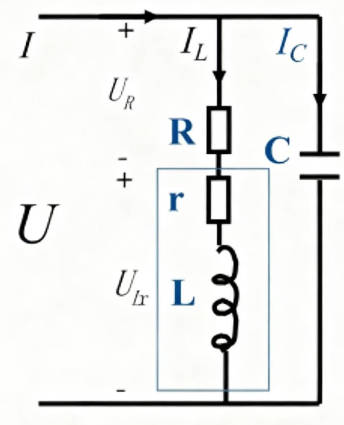
\includegraphics[width=0.4\textwidth]{figures/1.jpg}
        \caption{含不同负载及补偿电容的交流电路模型}
        \label{fig:rlc_circuit}
    \end{figure}

    根据相量分析，电容电流 $\dot{I}_C$ 超前电压 $90^\circ$，而感性支路电流 $\dot{I}_L$ 滞后电压。通过并联电容，$\dot{I}_C$ 可以抵消部分感性无功电流分量，使得总电流 $\dot{I}$ 减小，相位差 $\varphi$ 变小，从而提高功率因数 $\cos\varphi$。值得注意的是，补偿应当适度，若电容过大（过补偿），电路将呈容性，功率因数反而会下降。
\end{enumerate}

\subsection{实验方法}
本实验旨在通过实际测量验证上述原理，具体操作步骤如下：

\begin{enumerate}
    \item 构建基础电路：
    按图示连接日光灯实验电路。在未接入补偿电容前，闭合总电源开关及日光灯开关，观察日光灯辉光放电及启辉器的工作过程，直至灯管稳定发光。

    \item 基准参数测量：
    使用功率表、交流电压表和电流表，测量日光灯在额定电压工作时的有功功率 $P$、电压 $U$ 和电流 $I$。利用公式 $\cos\varphi = P/(UI)$ 计算未补偿时的功率因数。

    \item 电容补偿测试：
    在电路中并联电容器箱，按照电容值从小到大（例如 $1\mu F, 2.2\mu F, 4.7\mu F \dots$）的顺序调节。
    \begin{itemize}
        \item 逐次测量并记录不同电容值下的总电流 $I$、电压 $U$ 和有功功率 $P$。
        \item 重点捕捉总电流达到最小值时的电容值，此时即为最佳补偿状态。
    \end{itemize}

    \item 数据处理与分析：
    根据记录的数据计算各组的功率因数，并绘制 $\cos\varphi - C$ 关系散点图，直观分析功率因数随电容变化的非单调性规律。
\end{enumerate}

\subsection{实验现象}
\begin{enumerate}
    \item 启动过程：日光灯启动时，启辉器内双金属片断开瞬间产生高压脉冲，使灯管内气体电离，产生辉光放电，灯光由暗逐渐变亮并稳定。
    
    \item 参数变化规律：
    \begin{itemize}
        \item 未接电容时：测得电路总电流较大，计算出的功率因数较低（通常在 0.5 左右）。
        \item 增加电容过程中：随着并联电容值 $C$ 的增加，总电流 $I$ 呈现“先减小后增大”的趋势；而功率因数 $\cos\varphi$ 则呈现“先升高后降低”的趋势。
        \item 最佳补偿点：当电容值达到某一特定值时，总电流最小，功率因数达到最大值（接近 1.0）。此时电路呈纯阻性，电能利用率最高。若继续增大电容，电路变为容性，总电流重新增大，功率因数下降。
    \end{itemize}
\end{enumerate}

\newpage

% ======================================================================
% 第二部分：组装整流器实验
% ======================================================================
\section{组装整流器实验}

\subsection{实验原理}
整流电路利用二极管的单向导电特性，将交变电压（AC）转换为脉动直流电压（DC）。

\begin{enumerate}
    \item 整流电路拓扑：
    \begin{itemize}
        \item 单相半波整流（图 \ref{fig:1}）：利用一只二极管，仅截取交流电的正半周，输出电压平均值低（$U_o \approx 0.45U_2$），效率较低。
        \item 单相全波整流（图 \ref{fig:2}）：利用带中心抽头的变压器和两只二极管，正负半周轮流导通。
        \item 桥式整流（图 \ref{fig:3}）：利用四只二极管组成的电桥，实现了全波整流且无需中心抽头变压器，输出电压平均值高（$U_o \approx 0.9U_2$），是应用最广泛的整流电路。
    \end{itemize}

    \begin{figure}[H]
        \centering
        \begin{minipage}[t]{0.45\linewidth}
            \centering
            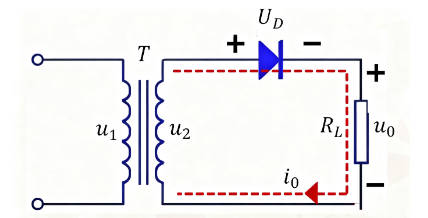
\includegraphics[width=0.8\textwidth]{figures/2.jpg}
            \caption{单相半波整流电路}
            \label{fig:1}
        \end{minipage}
        \begin{minipage}[t]{0.45\linewidth}
            \centering
            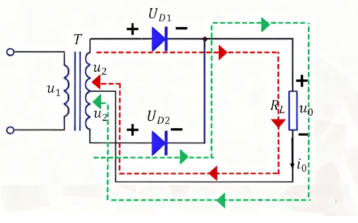
\includegraphics[width=0.8\textwidth]{figures/3.jpg}
            \caption{单相全波整流电路}
            \label{fig:2}
        \end{minipage}
    \end{figure}

    \begin{figure}[H]
        \centering
        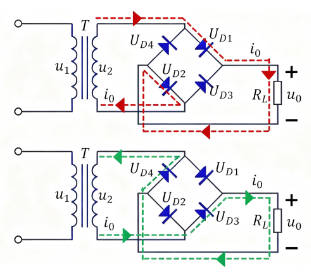
\includegraphics[width=0.4\textwidth]{figures/4.jpg}
        \caption{桥式整流电路}
        \label{fig:3}
    \end{figure}
    \item 滤波原理：
    整流后的电压虽然方向单一，但大小随时间脉动。在负载两端并联电容 $C$ 构成 RC 滤波电路。利用电容“电压不能突变”的储能特性：
    \begin{itemize}
        \item 当电源电压升高时，二极管导通，电源给电容充电；
        \item 当电源电压降低时，二极管截止，电容向负载放电，填补电压低谷。
    \end{itemize}
    放电时间常数 $\tau = R_L C$ 越大，输出波形越平滑，越接近理想直流电。
    滤波电路如图 \ref{fig:filter} 所示。
    \begin{figure}[H]
        \centering
        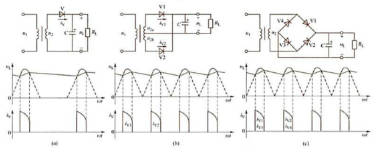
\includegraphics[width=0.8\textwidth]{figures/5.jpg}
        \caption{含不同负载及补偿电容的交流电路模型}
        \label{fig:filter}
    \end{figure}
\end{enumerate}

\subsection{实验方法}
\begin{enumerate}
    \item 电路搭建与波形观测：
    分别在实验板上搭建单相半波、全波及桥式整流电路。使用双踪示波器，通道1监测变压器副边输入交流波形，通道2监测负载两端的输出波形。

    \item 参数测量：
    利用示波器的测量功能，记录三种整流电路的以下参数：
    \begin{itemize}
        \item 输入信号有效值 $U_2$；
        \item 输出信号的有效值 $U_o$ 和平均值 $\overline{U_o}$；
        \item 二极管承受的反向峰值电压 $U_{Rmax}$。
    \end{itemize}

    \item 滤波效果对比：
    保持整流电路不变，分别在负载两端并联 $47\mu F$ 和 $470\mu F$ 的电解电容（注意极性不能接反）。观察并描绘不同电容值下，输出电压纹波幅度的变化情况。
\end{enumerate}

\subsection{实验现象}
\begin{enumerate}
    \item 波形特征：
    \begin{itemize}
        \item 半波整流：输出为断续的单向脉冲，有一半时间电压为零。
        \item 全波/桥式整流：输出为连续的单向脉冲，脉动频率是输入频率的2倍。
    \end{itemize}

    \item 滤波效果分析：
    \begin{itemize}
        \item 未加电容时：输出波形起伏剧烈，脉动系数大。
        \item 接入小电容（$47\mu F$）后：波形由脉冲状变为锯齿状，脉动幅度明显减小，平均电压提升。
        \item 接入大电容（$470\mu F$）后：由于充放电时间常数显著增大，电容放电极慢，输出波形变得非常平滑，仅存极微小的纹波，已十分接近理想直流电源。
    \end{itemize}
\end{enumerate}

\newpage

% ======================================================================
% 第三部分：实验重点
% ======================================================================
\section{实验重点}

\subsection{交流电路功率因数实验}
\begin{itemize}
    \item 概念理解：深入理解功率因数 $\cos\varphi = P/S$ 的物理意义，明确它代表了电源容量被转化为有用功的比例。
    \item 相位特性：掌握感性负载（如日光灯）中“电流滞后电压”的相位特性，以及通过相量图分析电压与电流关系的方法。
    \item 补偿规律：掌握“并联电容补偿无功功率”的原理，重点观测并分析电容容量变化对总电流及功率因数的影响规律（即倒U型曲线），理解过补偿的危害。
\end{itemize}

\subsection{组装整流器实验}
\begin{itemize}
    \item 电路机理：熟练掌握半波、全波、桥式三种整流电路的结构差异，明确二极管的导通逻辑与电流路径。
    \item 滤波机制：理解电容滤波的“充放电”机制，对比分析不同容值（$47\mu F$ vs $470\mu F$）对整流输出波形平滑效果的显著差异。
    \item 仪器使用：能够熟练使用数字示波器（特别是直流耦合 DC Coupling 模式）观察整流与滤波波形，并准确读取输入有效值、输出平均值及二极管反向峰值电压。
\end{itemize}

% ======================================================================
% 第四部分：实验难点
% ======================================================================
\section{实验难点}

\subsection{交流电路功率因数实验}
\begin{itemize}
    \item 相位差的测量与判断：在示波器上观测时，初学者较难结合李萨如图形或双踪波形准确区分“电流超前”还是“电流滞后”于电压，容易混淆相位关系。
    \item 临界点的准确捕捉：功率因数随电容变化呈非线性规律，在实验中寻找电流最小值（即功率因数最大值）对应的准确电容值较为困难，且数据测量误差容易导致规律曲线发生偏移，影响对“过补偿”现象的判断。
\end{itemize}

\subsection{组装整流器实验}
\begin{itemize}
    \item 波形参数的精确读取：整流后的波形属于非正弦周期信号，示波器上显示的“峰值”、“有效值”和“平均值”物理意义不同，学生容易在读取数据时产生混淆，导致计算误差。
    \item 频率与滤波关系的理解：需结合理论理解半波（$50Hz$ 脉动）与全波（$100Hz$ 脉动）在相同滤波电容下的效果差异，难点在于构建“脉动频率越高，电容放电越少，滤波效果越好”的逻辑关联。
\end{itemize}



\begin{fullreportonly}
\section{原始数据（20分）}
（将有老师签名的“自备数据记录草稿纸”的扫描或手机拍摄图粘贴在下方，完整保留姓名，学号，教师签字和日期。）
\begin{figure}[H]
    \centering
    
\includegraphics[width=0.8\textwidth]{figures/原始数据.jpg}
    \caption{原始数据记录}
    \label{fig:原始数据}
\end{figure}

\section{结果与分析}

\subsection{数据处理与结果}

\subsubsection{1.1 交流电路功率因数实验数据处理}

根据实验测量数据，记录电容 $C$、电流 $I$、电压 $U$ 和功率 $P$。功率因数 $\cos\varphi$ 由公式 $\cos\varphi = \frac{P}{UI}$ 计算得出。

\begin{table}[H]
    \centering
    \caption{交流电路实验数据记录与计算}
    \label{tab:ac_data}
    \begin{tabular}{cccccc}
        \toprule
        \textbf{类别} & $C / \mu \text{F}$ & $I / \text{mA}$ & $U / \text{V}$ & $P / \text{W}$ & $\cos\varphi$ (计算值) \\
        \midrule
        未加电容 & 0 & 291.0 & 216.1 & 21.5 & 0.3419 \\
        加电容 & 1 & 234.4 & 216.1 & 21.8 & 0.4304 \\
        加电容 & 2 & 202.6 & 216.2 & 22.0 & 0.5022 \\
        加电容 & 3 & 145.8 & 216.4 & 22.2 & 0.7036 \\
        加电容 & 4 & 126.3 & 216.4 & 22.4 & 0.8196 \\
        加电容 & 5 & 136.9 & 216.7 & 22.5 & 0.7584 \\
        加电容 & 6 & 156.1 & 216.4 & 22.4 & 0.6631 \\
        加电容 & 7 & 203.8 & 216.4 & 22.6 & 0.5124 \\
        加电容 & 8 & 255.6 & 216.4 & 22.6 & 0.4086 \\
        加电容 & 9 & 317.2 & 216.4 & 22.7 & 0.3307 \\
        \bottomrule
    \end{tabular}
\end{table}

% 功率因数拟合曲线参数
\def\Cmax{4.3313}
\def\cosphimax{0.8592}
\def\fitfunc{-0.000394*x^5 + 0.011656*x^4 - 0.123739*x^3 + 0.544662*x^2 - 0.848508*x + 0.869792}

\textbf{实验曲线图与数据拟合：}

下图为I、U、P随C变化曲线。重点对功率因数 $\cos\varphi$ 随电容 $C$ 变化的数据进行五次多项式拟合，拟合函数为：
$$ \cos\varphi = -0.000394C^5 + 0.011656C^4 - 0.123739C^3 + 0.544662C^2 - 0.848508C + 0.869792 $$
根据拟合曲线，最大功率因数对应的电容值为 $\approx \Cmax \mu\text{F}$，最大功率因数为 $\approx \cosphimax$。

\begin{figure}[H]
    \centering
    % 第一行：I-C 和 U-C
    \begin{subfigure}[b]{0.45\textwidth}
        \centering
        \begin{tikzpicture}[scale=0.6]
            \begin{axis}[xlabel={C($\mu$F)}, ylabel={I(mA)}, grid=major, title={电流 I 随电容变化}]
            \addplot[mark=*, blue] coordinates {(0,291.0) (1,234.4) (2,202.6) (3,145.8) (4,126.3) (5,136.9) (6,156.1) (7,203.8) (8,255.6) (9,317.2)};
            \end{axis}
        \end{tikzpicture}
    \end{subfigure}
    \hfill
    \begin{subfigure}[b]{0.45\textwidth}
        \centering
        \begin{tikzpicture}[scale=0.6]
            \begin{axis}[xlabel={C($\mu$F)}, ylabel={U(V)}, grid=major, title={电压 U 随电容变化}, y tick label style={/pgf/number format/.cd,fixed,fixed zerofill,precision=1}]
            \addplot[mark=*, blue] coordinates {(0,216.1) (1,216.1) (2,216.2) (3,216.4) (4,216.4) (5,216.7) (6,216.4) (7,216.4) (8,216.4) (9,216.4)};
            \end{axis}
        \end{tikzpicture}
    \end{subfigure}
    
    \vspace{0.5cm}
    
    % 第二行：P-C 和 cosphi拟合
    \begin{subfigure}[b]{0.45\textwidth}
        \centering
        \begin{tikzpicture}[scale=0.6]
            \begin{axis}[xlabel={C($\mu$F)}, ylabel={P(W)}, grid=major, title={功率 P 随电容变化}]
            \addplot[mark=*, blue] coordinates {(0,21.5) (1,21.8) (2,22.0) (3,22.2) (4,22.4) (5,22.5) (6,22.4) (7,22.6) (8,22.6) (9,22.7)};
            \end{axis}
        \end{tikzpicture}
    \end{subfigure}
    \hfill
    \begin{subfigure}[b]{0.45\textwidth}
        \centering
        \begin{tikzpicture}[scale=0.6]
            \begin{axis}[
                xlabel={C($\mu$F)}, ylabel={$\cos\varphi$}, grid=major, title={功率因数拟合},
                xmin=-0.5, xmax=9.5, ymin=0.3, ymax=0.9
            ]
            \addplot[mark=*, only marks, red] coordinates {(0,0.3419) (1,0.4304) (2,0.5022) (3,0.7036) (4,0.8196) (5,0.7584) (6,0.6631) (7,0.5124) (8,0.4086) (9,0.3307)};
            \addplot[blue, thick, domain=0:9, samples=100] {\fitfunc};
            \addplot[mark=star, green, mark size=4pt] coordinates {(\Cmax,\cosphimax)};
            \end{axis}
        \end{tikzpicture}
    \end{subfigure}
    \caption{交流电路实验曲线}
\end{figure}

\subsubsection{1.2 组装整流器实验数据处理}

实验测得三种整流电路在无滤波电容情况下的数据如下表所示：

\begin{table}[H]
    \centering
    \caption{整流器实验数据（无滤波器）}
    \label{tab:rectifier_data}
    \begin{tabular}{lccccc}
        \toprule
        \textbf{整流电路类型} & \textbf{$U_2$ 峰峰值/V} & \textbf{$U_2$ 有效值/V} & \textbf{$U_o$ 平均值/V} & \textbf{$U_d$/V (正向)} & \textbf{$U_{Rmax}$/V (反向)} \\
        \midrule
        单相半波整流 & 17.60 & 3.951 & 2.319 & 10.40 & 10.75 \\
        单相全波整流 & 18.93 & 5.540 & 4.827 & 18.93 & 19.20 \\
        桥式整流电路 & 18.96 & 5.186 & 4.466 & 9.652 & 9.620 \\
        \bottomrule
    \end{tabular}
\end{table}

\textbf{整流电路波形图：}

\noindent \textbf{1. 单相半波整流电路}

\begin{figure}[H]
    \centering
    \begin{subfigure}[b]{0.45\textwidth}
        \centering
        
\includegraphics[width=\linewidth, height=3.5cm, keepaspectratio]{half_u2.jpg}
        \caption{输入信号 $U_2$}
    \end{subfigure}
    \hfill
    \begin{subfigure}[b]{0.45\textwidth}
        \centering
        
\includegraphics[width=\linewidth, height=3.5cm, keepaspectratio]{half_u0.jpg}
        \caption{输出信号 $U_0$}
    \end{subfigure}
    \vspace{0.2cm}
    \begin{subfigure}[b]{0.45\textwidth}
        \centering
        
\includegraphics[width=\linewidth, height=3.5cm, keepaspectratio]{half_diode_fwd.jpg}
        \caption{二极管正向电压}
    \end{subfigure}
    \hfill
    \begin{subfigure}[b]{0.45\textwidth}
        \centering
        
\includegraphics[width=\linewidth, height=3.5cm, keepaspectratio]{half_diode_rev.jpg}
        \caption{二极管反向电压}
    \end{subfigure}
    \caption{单相半波整流电路波形}
\end{figure}

\noindent \textbf{2. 单相全波整流电路}

\begin{figure}[H]
    \centering
    \begin{subfigure}[b]{0.45\textwidth}
        \centering
        
\includegraphics[width=\linewidth, height=3.5cm, keepaspectratio]{full_u2.jpg}
        \caption{输入信号 $U_2$}
    \end{subfigure}
    \hfill
    \begin{subfigure}[b]{0.45\textwidth}
        \centering
        
\includegraphics[width=\linewidth, height=3.5cm, keepaspectratio]{full_u0.jpg}
        \caption{输出信号 $U_0$}
    \end{subfigure}
    \vspace{0.2cm}
    \begin{subfigure}[b]{0.45\textwidth}
        \centering
        
\includegraphics[width=\linewidth, height=3.5cm, keepaspectratio]{full_diode_fwd.jpg}
        \caption{二极管正向电压}
    \end{subfigure}
    \hfill
    \begin{subfigure}[b]{0.45\textwidth}
        \centering
        
\includegraphics[width=\linewidth, height=3.5cm, keepaspectratio]{full_diode_rev.jpg}
        \caption{二极管反向电压}
    \end{subfigure}
    \caption{单相全波整流电路波形}
\end{figure}

\noindent \textbf{3. 桥式整流电路}

\begin{figure}[H]
    \centering
    \begin{subfigure}[b]{0.45\textwidth}
        \centering
        
\includegraphics[width=\linewidth, height=3.5cm, keepaspectratio]{bridge_u2.jpg}
        \caption{输入信号 $U_2$}
    \end{subfigure}
    \hfill
    \begin{subfigure}[b]{0.45\textwidth}
        \centering
        
\includegraphics[width=\linewidth, height=3.5cm, keepaspectratio]{bridge_u0.jpg}
        \caption{输出信号 $U_0$}
    \end{subfigure}
    \vspace{0.2cm}
    \begin{subfigure}[b]{0.45\textwidth}
        \centering
        
\includegraphics[width=\linewidth, height=3.5cm, keepaspectratio]{bridge_diode_fwd.jpg}
        \caption{二极管正向电压}
    \end{subfigure}
    \hfill
    \begin{subfigure}[b]{0.45\textwidth}
        \centering
        
\includegraphics[width=\linewidth, height=3.5cm, keepaspectratio]{bridge_diode_rev.jpg}
        \caption{二极管反向电压}
    \end{subfigure}
    \caption{桥式整流电路波形}
\end{figure}

\noindent \textbf{3. 滤波电路}
给桥式整流电路加上滤波电容，得到不同电容值的输出波形如下：
\begin{figure}[H]
    \centering
    \begin{subfigure}[b]{0.45\textwidth}
        \centering
        
\includegraphics[width=\linewidth, height=3.5cm, keepaspectratio]{0.47.jpg}
        \caption{C=0.47uF}
    \end{subfigure}
    \hfill
    \begin{subfigure}[b]{0.45\textwidth}
        \centering
        
\includegraphics[width=\linewidth, height=3.5cm, keepaspectratio]{47.jpg}
        \caption{C=47uF}
    \end{subfigure}
    \vspace{0.2cm}
    \begin{subfigure}[b]{0.45\textwidth}
        \centering
        
\includegraphics[width=\linewidth, height=3.5cm, keepaspectratio]{470.jpg}
        \caption{C=470uF}
    \end{subfigure}
    \hfill
    \begin{subfigure}[b]{0.45\textwidth}
        \centering
        
\includegraphics[width=\linewidth, height=3.5cm, keepaspectratio]{1000.jpg}
        \caption{C=1000uF}
    \end{subfigure}
    \caption{桥式整流滤波电路输出波形}
\end{figure}
可见滤波电容越大，输出波形越平滑，纹波幅度越小，滤波效果越好。
\section{误差分析}

\subsection{2.1 交流电路功率因数实验误差分析}

\subsubsection{误差原因分析}
\begin{enumerate}
    \item \textbf{非线性负载特性}：日光灯内含镇流器，工作时产生高次谐波，导致电压电流波形畸变，偏离标准正弦波，使得基于 $\cos\varphi = P/UI$ 的计算存在原理性偏差。
    \item \textbf{电网波动}：实验过程中电网电压存在微小波动，导致电压、电流和功率读数不同步。
    \item \textbf{仪表接入误差}：功率表电流线圈和电压线圈的接入方式会引入分压或分流误差。
\end{enumerate}

\subsubsection{功率因数不确定度分析}
功率因数 $\lambda = \cos\varphi = \frac{P}{U \cdot I}$。根据不确定度传播定律，相对标准不确定度 $u_r(\lambda)$ 可由下式计算：
$$ u_r(\lambda) = \sqrt{u_r(P)^2 + u_r(U)^2 + u_r(I)^2} $$
\textbf{计算示例（取 $C=4\mu\text{F}$ 数据点）：}
$P=22.4\text{W}, U=216.4\text{V}, I=126.3\text{mA}=0.1263\text{A}$。
假设使用0.5级仪表，取置信因子 $k=\sqrt{3}$（均匀分布），则仪器引入的相对标准不确定度约为 $u_r \approx \frac{0.5\%}{\sqrt{3}} \approx 0.29\%$。
$$ u_r(\lambda) = \sqrt{0.29\%^2 + 0.29\%^2 + 0.29\%^2} \approx 0.5\% $$
此时功率因数计算值为 $0.8196$，则其标准不确定度为：
$$ u(\lambda) = 0.8196 \times 0.5\% \approx 0.0041 $$
即 $\cos\varphi = 0.8196 \pm 0.0041$ (仅考虑B类不确定度)。

\subsection{2.2 滤波电路实验误差分析}

\subsubsection{整流电路实验系数与误差计算}
基于公式 $k_{\text{实验}} = \frac{U_o}{U_2}$ 计算实验系数，并与理论标准系数（半波0.45，全波/桥式0.9）进行比较。

\paragraph{1. 单相半波整流电路}
\begin{itemize}
    \item 实验数据：$U_2 = 3.951\text{V}, U_o = 2.319\text{V}$
    \item 实验系数：$k_{\text{实验}} = \frac{2.319}{3.951} \approx 0.5869$
    \item 绝对误差：$|k_{\text{实验}} - k_{\text{标准}}| = |0.5869 - 0.45| = 0.1369$
    \item 相对误差：$\frac{0.1369}{0.45} \times 100\% \approx 30.42\%$
\end{itemize}

\paragraph{2. 单相全波整流电路}
\begin{itemize}
    \item 实验数据：$U_2 = 5.540\text{V}, U_o = 4.827\text{V}$
    \item 实验系数：$k_{\text{实验}} = \frac{4.827}{5.540} \approx 0.8713$
    \item 绝对误差：$|k_{\text{实验}} - k_{\text{标准}}| = |0.8713 - 0.9| = 0.0287$
    \item 相对误差：$\frac{0.0287}{0.9} \times 100\% \approx 3.19\%$
\end{itemize}

\paragraph{3. 桥式整流电路}
\begin{itemize}
    \item 实验数据：$U_2 = 5.186\text{V}, U_o = 4.466\text{V}$
    \item 实验系数：$k_{\text{实验}} = \frac{4.466}{5.186} \approx 0.8612$
    \item 绝对误差：$|k_{\text{实验}} - k_{\text{标准}}| = |0.8612 - 0.9| = 0.0388$
    \item 相对误差：$\frac{0.0388}{0.9} \times 100\% \approx 4.31\%$
\end{itemize}

\subsubsection{整流电压不确定度分析}
假设使用数字万用表进行电压测量，准确度为 $\pm(0.5\% \text{读数} + 2\text{字})$。以桥式整流电路数据为例进行 B 类不确定度评定。

\textbf{1. 输入电压 $U_2$ 的不确定度}
\begin{itemize}
    \item 读数 $U_2 = 5.186\text{V}$。
    \item 最大允许误差 $\Delta_{U2} = 5.186 \times 0.5\% + 0.002 \approx 0.028\text{V}$。
    \item 标准不确定度 $u(U_2) = \frac{\Delta_{U2}}{\sqrt{3}} = \frac{0.028}{1.732} \approx 0.016\text{V}$。
\end{itemize}

\textbf{2. 输出电压 $U_o$ 的不确定度}
\begin{itemize}
    \item 读数 $U_o = 4.466\text{V}$。
    \item 最大允许误差 $\Delta_{Uo} = 4.466 \times 0.5\% + 0.002 \approx 0.024\text{V}$。
    \item 标准不确定度 $u(U_o) = \frac{\Delta_{Uo}}{\sqrt{3}} = \frac{0.024}{1.732} \approx 0.014\text{V}$。
\end{itemize}

\textbf{3. 实验系数 $k$ 的合成不确定度}
由 $k = \frac{U_o}{U_2}$，相对标准不确定度为：
$$ u_r(k) = \sqrt{\left(\frac{u(U_o)}{U_o}\right)^2 + \left(\frac{u(U_2)}{U_2}\right)^2} $$
$$ u_r(k) = \sqrt{\left(\frac{0.014}{4.466}\right)^2 + \left(\frac{0.016}{5.186}\right)^2} \approx \sqrt{0.0031^2 + 0.0031^2} \approx 0.44\% $$
故实验系数的标准不确定度 $u(k) = 0.8612 \times 0.44\% \approx 0.0038$。
$$ k_{\text{实验}} = 0.8612 \pm 0.0038 $$

\subsubsection{误差总结}
全波和桥式整流的相对误差较小（约 3\%-4\%），主要由二极管导通压降（约0.7V/管）引起；半波整流误差较大（约 30\%），主要归因于输出波形脉动过大导致的平均值测量误差，且不确定度分析表明仪器本身的随机误差不足以解释此偏差，确认为系统误差。


\section{实验探讨}

\subsection{3.1 交流电路功率因数实验探讨}
本实验深入验证了并联电容器对感性负载进行无功补偿的原理。
\begin{itemize}
    \item 物理机制验证：实验数据清晰展示了随着电容 $C$ 的增加，电路总电流呈现显著的“V”型变化规律。这验证了电容器产生的容性电流与电感性负载的感性电流在相位上互差 $180^\circ$，两者相互抵消，从而减小了从电网汲取的总无功电流。
    \item 欠补偿与过补偿：实验结果表明，在 $C \approx 4.33\mu\text{F}$ 时功率因数达到峰值，电路接近纯电阻性。当 $C$ 过大时，电路从感性转变为容性（过补偿），此时虽然有功功率 $P$ 变化不大，但视在功率 $S$ 增加，导致无功电流再次增大，造成功率因数恶化。
    \item 实际意义：通过实验深刻理解了提高功率因数对于降低线路损耗、提高变压器利用率以及改善电网电压质量的重要工程意义。
\end{itemize}

\subsection{3.2 整流与滤波电路实验探讨}
\begin{itemize}
    \item 整流电路性能对比：通过对比波形和数据，桥式整流在电压利用率和二极管反向耐压要求上展现出最佳的综合性能。虽然使用了4个二极管，但它不需要中心抽头变压器，且输出纹波频率是电源频率的2倍，易于滤波。
    \item 滤波效果分析：接入 $47\mu\text{F}$ 电容后，输出电压显著升高且波形趋于平滑。这验证了电容利用其“储能”特性，在电压下降阶段向负载放电，从而填补了脉动电压的谷底。这也启示我们在设计电源时，需要根据负载电流大小选择合适的时间常数 $\tau = R_L C$，以确保 $\tau \geq (3\sim5) \frac{T}{2}$，从而获得理想的直流电压。
\end{itemize}

\section{思考题}

\subsection*{1. 提高功率因数的意义何在？为什么并联电容能提高功率因数？并联的电容是否越大越好？}
\begin{enumerate}
    \item \textbf{提高功率因数的意义}：
    \begin{itemize}
        \item \textbf{提高能源利用率}：发电和输电设备的容量是按视在功率 $S$ 设计的。提高 $\cos\varphi$ 可以使设备在额定容量下输出更多的有功功率 $P$。
        \item \textbf{降低线路损耗}：在传输相同有功功率的情况下，电流 $I = P/(U\cos\varphi)$。功率因数越高，线路电流越小，线路上的热损耗 ($I^2R$) 越低。
        \item \textbf{改善电压质量}：减小线路压降，使负载端的电压更稳定。
    \end{itemize}
    \item \textbf{并联电容原理}：感性负载（如电机、日光灯）需要从电网吸收滞后的无功电流建立磁场。并联电容器后，电容产生超前的无功电流。两者在电路内部进行能量交换，减少了电源与负载之间无功功率的往复流动，从而降低了总电流。
    \item \textbf{并非越大越好}：若电容过大，无功电流会“反向”增大（容性电流占主导），不仅重新降低功率因数，还会导致线路末端电压升高（费兰梯效应），可能损坏绝缘或烧毁设备。最佳状态通常是将功率因数补偿到 0.9 - 0.95 左右，而非完全补偿到 1。
\end{enumerate}

\subsection*{2. 在实验中，随着电容增加，电路总电流的变化规律为由大变小再变大，试分析原因}
该现象反映了电路总阻抗随电容变化的谐振特性：
\begin{itemize}
    \item 初始阶段（欠补偿）：电路呈感性，感性无功电流 $I_L$ 大于容性无功电流 $I_C$。随着电容 $C$ 增加，$I_C$ 增大并抵消部分 $I_L$，总电流向量长度减小。
    \item 谐振点（完全补偿）：当电容增加到特定值时，感性分量与容性分量近似相等，电路发生并联谐振，总阻抗最大，总电流达到最小值。
    \item 后期阶段（过补偿）：电容继续增加，$I_C$ 超过 $I_L$，电路呈容性。随着 $C$ 增大，容抗 $X_C$ 减小，容性电流剧增，导致总电流再次变大。
\end{itemize}

\subsection*{3. 在进行功率因数补偿时，本实验采用并联电容器的方法，为什么不采用串联电容器的方法？}
\begin{itemize}
    \item \textbf{电压稳定性（核心原因）}：并联电容不改变负载两端的电压，保证负载（如日光灯）在额定电压下正常工作。若采用串联，电容会分担部分电压，导致负载两端电压降低，无法正常启动或亮度不足。
    \item \textbf{避免串联谐振}：串联电容器容易与感性负载发生电压谐振，可能在电感或电容两端产生数倍于电源电压的高压，严重威胁人身安全和设备绝缘。
    \item \textbf{操作灵活性}：并联补偿可以根据负荷变化灵活投入或切除电容器，互不影响。
\end{itemize}

\subsection*{4. 总结不同的整流电路和不同滤波电路的利弊}
\begin{itemize}
    \item \textbf{单相半波整流}：
    \begin{itemize}
        \item \textbf{利}：电路极其简单，仅需1只二极管。
        \item \textbf{弊}：输出电压低 ($0.45U_2$)，脉动极大，变压器利用率低且存在直流磁化问题。仅适用于小电流、要求不高的场合。
    \end{itemize}
    \item \textbf{单相全波整流}：
    \begin{itemize}
        \item \textbf{利}：输出电压较高 ($0.9U_2$)，整流效率高。
        \item \textbf{弊}：二极管承受反向电压高 ($2\sqrt{2}U_2$)，且必须使用带中心抽头的特制变压器。
    \end{itemize}
    \item \textbf{桥式整流}：
    \begin{itemize}
        \item \textbf{利}：输出电压高，二极管反向耐压要求低 ($\sqrt{2}U_2$)，变压器利用率最高。
        \item \textbf{弊}：使用了4只二极管，导通压降相对较大（两倍管压降），结构略复杂。但它是目前最主流的整流方案。
    \end{itemize}
\end{itemize}

\subsection*{5. 整流和滤波的目的是什么？}
\begin{itemize}
    \item \textbf{整流}：利用二极管的单向导电性，将方向和大小随时间变化的正弦交流电（AC）转换为方向不变、但大小仍随时间脉动的直流电（Pulsating DC）。
    \item \textbf{滤波}：利用电容（储能）或电感（阻碍电流变化）的特性，滤除整流输出电压中的交流谐波分量，填补波谷，削弱波峰，将脉动直流电转变为平滑、稳定的直流电，以接近电池的输出特性。
\end{itemize}

\subsection*{6. 如何根据需要选择合适的整流电路？}
选择时需综合考虑以下工程因素：
\begin{itemize}
    \item \textbf{负载对纹波的要求}：若要求低纹波、高稳定性，首选桥式整流配合 $\pi$ 型滤波；若要求不高（如简易充电器），可选半波整流。
    \item \textbf{输出电压与功率}：高压小电流场合（如显像管高压）多用倍压整流；大功率场合多用桥式整流以提高变压器效率。
    \item \textbf{元件耐压限制}：若二极管耐压受限，应避免使用全波整流（需承受2倍反压），改用桥式整流。
    \item \textbf{成本与体积}：半波整流成本最低，但在滤波环节可能需要更大的电容，需权衡整体体积。
\end{itemize}



\end{fullreportonly}
\insertnotes
\end{document}